%%%%%%%%%%%%%%%%%%%%%%%%%%%%%%%%%%%
%This is the LaTeX ARTICLE template for RSC journals
%Copyright The Royal Society of Chemistry 2014
%%%%%%%%%%%%%%%%%%%%%%%%%%%%%%%%%%%

\documentclass[twoside,twocolumn,9pt]{article}
\usepackage{extsizes}
\usepackage[super,sort&compress,comma]{natbib} 
\usepackage[version=3]{mhchem}
\usepackage[left=1.5cm, right=1.5cm, top=1.785cm, bottom=2.0cm]{geometry}
\usepackage{balance}
\usepackage{widetext}
\usepackage{times,mathptmx}
\usepackage{sectsty}
\usepackage{graphicx} 
\usepackage{subcaption}
\usepackage{mwe}
\usepackage{float}
\usepackage{lastpage}
\usepackage[format=plain,justification=raggedright,singlelinecheck=false,font={stretch=1.125,small,sf},labelfont=bf,labelsep=space]{caption}
\usepackage{float}
\usepackage{fancyhdr}
\usepackage{fnpos}
\usepackage[english]{babel}
\usepackage{array}
\usepackage{droidsans}
\usepackage{charter}
\usepackage[T1]{fontenc}
\usepackage[usenames,dvipsnames]{xcolor}
\usepackage{setspace}
\usepackage[compact]{titlesec}
%%%Please don't disable any packages in the preamble, as this may cause the template to display incorrectly.%%%


\usepackage{epstopdf}%This line makes .eps figures into .pdf - please comment out if not required.

\definecolor{cream}{RGB}{222,217,201}

\begin{document}

\pagestyle{fancy}
\thispagestyle{plain}
\fancypagestyle{plain}{

%%%HEADER%%%
\fancyhead[C]{
\includegraphics[width=18.5cm]{header_bar.pdf}}
\fancyhead[L]{\hspace{0cm}\vspace{1.5cm}\LARGE QuantBio Express}
%\fancyhead[L]{\hspace{0cm}\vspace{1.5cm}\includegraphics[height=30pt]{head_foot/journal_name}}
\fancyhead[R]{\hspace{0cm}\vspace{2.5cm}}
%\fancyhead[R]{\hspace{0cm}\vspace{1.7cm}\includegraphics[height=55pt]{head_foot/RSC_LOGO_CMYK}}
\renewcommand{\headrulewidth}{0pt}
}
%%%END OF HEADER%%%

%%%PAGE SETUP - Please do not change any commands within this section%%%
\makeFNbottom
\makeatletter
\renewcommand\LARGE{\@setfontsize\LARGE{15pt}{17}}
\renewcommand\Large{\@setfontsize\Large{12pt}{14}}
\renewcommand\large{\@setfontsize\large{10pt}{12}}
\renewcommand\footnotesize{\@setfontsize\footnotesize{7pt}{10}}
\makeatother

\renewcommand{\thefootnote}{\fnsymbol{footnote}}
\renewcommand\footnoterule{\vspace*{1pt}% 
\color{cream}\hrule width 3.5in height 0.4pt \color{black}\vspace*{5pt}} 
\setcounter{secnumdepth}{5}

\makeatletter 
\renewcommand\@biblabel[1]{#1}            
\renewcommand\@makefntext[1]% 
{\noindent\makebox[0pt][r]{\@thefnmark\,}#1}
\makeatother 
\renewcommand{\figurename}{\small{Fig.}~}
\sectionfont{\sffamily\Large}
\subsectionfont{\normalsize}
\subsubsectionfont{\bf}
\setstretch{1.125} %In particular, please do not alter this line.
\setlength{\skip\footins}{0.8cm}
\setlength{\footnotesep}{0.25cm}
\setlength{\jot}{10pt}
\titlespacing*{\section}{0pt}{4pt}{4pt}
\titlespacing*{\subsection}{0pt}{15pt}{1pt}
%%%END OF PAGE SETUP%%%

%%%FOOTER%%%
\fancyfoot{}
\fancyfoot[LO,RE]{\vspace{-7.1pt}
\includegraphics[height=15pt]{cc-by-nc-sa.png}}
%\fancyfoot[CO]{\vspace{-7.1pt}\hspace{13.2cm}\includegraphics{head_foot/RF}}
\fancyfoot[CO]{\vspace{-7.1pt}QuantBio Express, vol. 1}
\fancyfoot[CE]{\vspace{-7.2pt}QuantBio Express, vol. 1}
%\fancyfoot[CE]{\vspace{-7.2pt}\hspace{-14.2cm}\includegraphics{head_foot/RF}}
\fancyfoot[RO]{\footnotesize{\sffamily{1--\pageref{LastPage} ~\textbar  \hspace{2pt}\thepage}}}
\fancyfoot[LE]{\footnotesize{\sffamily{\thepage~\textbar 1--\pageref{LastPage}}}}
\fancyhead{}
\renewcommand{\headrulewidth}{0pt} 
\renewcommand{\footrulewidth}{0pt}
\setlength{\arrayrulewidth}{1pt}
\setlength{\columnsep}{6.5mm}
\setlength\bibsep{1pt}
%%%END OF FOOTER%%%

%%%FIGURE SETUP - please do not change any commands within this section%%%
\makeatletter 
\newlength{\figrulesep} 
\setlength{\figrulesep}{0.5\textfloatsep} 

\newcommand{\topfigrule}{\vspace*{-1pt}% 
\noindent{\color{cream}\rule[-\figrulesep]{\columnwidth}{1.5pt}} }

\newcommand{\botfigrule}{\vspace*{-2pt}% 
\noindent{\color{cream}\rule[\figrulesep]{\columnwidth}{1.5pt}} }

\newcommand{\dblfigrule}{\vspace*{-1pt}% 
\noindent{\color{cream}\rule[-\figrulesep]{\textwidth}{1.5pt}} }

\makeatother
%%%END OF FIGURE SETUP%%%

%%%TITLE, AUTHORS AND ABSTRACT%%%
\twocolumn[
  \begin{@twocolumnfalse}
\vspace{3cm}
\sffamily


\noindent\LARGE{\textbf{Who turned out the lights: the shortcomings and successes of a Boolean network model for circadian processes$^\dag$}} \\%Article title goes here instead of the text "This is the title"

 \noindent\large{Adam Gruenbaum and Graham Northrup} \\%Author names go here instead of "Full name", etc.


\noindent\normalsize{The purpose of this paper is to stress test a Boolean network representing circadian rhythms of \textit{Arabidopsis thaliana}. We reproduced a Boolean model for these rhythms obtained from [O. E. Akman, Journal of The Royal Society, 2012.], and subjected the model to situations outside of the standard conditions under which it was designed. We tested it with a variety of photoperiods and submitted it to asynchronous behavior from the light inputs. We found that this particular model doesn't respond well to large changes in photoperiods, but does respond fairly well to asynchronous light node behavior. For a model so small (in terms of number of nodes) it is difficult to rectify these issues, however there are more complex models of the same system that might be more robust to change.} \\%The abstrast goes here instead of the text "The abstract should be..."


 \end{@twocolumnfalse} \vspace{0.6cm}

  ]
%%%END OF TITLE, AUTHORS AND ABSTRACT%%%

%%%FONT SETUP - please do not change any commands within this section
\renewcommand*\rmdefault{bch}\normalfont\upshape
\rmfamily
\section*{}
\vspace{-1cm}


%%%FOOTNOTES%%%

%Please use \dag to cite the ESI in the main text of the article.
%If you article does not have ESI please remove the the \dag symbol from the title and the footnotetext below.
\footnotetext{\dag~Electronic Supplementary Information (ESI) available: https://github.com/gnorthrup/BooleanControl}
%additional addresses can be cited as above using the lower-case letters, c, d, e... If all authors are from the same address, no letter is required

%\footnotetext{\ddag~Additional footnotes to the title and authors can be included \emph{e.g.}\ `Present address:' or `These authors contributed equally to this work' as above using the symbols: \ddag, \textsection, and \P. Please place the appropriate symbol next to the author's name and include a \texttt{\textbackslash footnotetext} entry in the the correct place in the list.}


%%%END OF FOOTNOTES%%%

%%%MAIN TEXT%%%%

\section{Introduction}

Biology is comprised of many processes regulated by the 24hr period of the day, temperature, or other environmental factors. These systems, circadian systems, typically stand on the back of gene regulatory networks (GRNs). A GRN is a group of genes linked by excitatory and inhibitory pathways which, in the circadian case, produce regulated, periodic outputs. These networks can be, and frequently are, modeled using ordinary differential equations (ODEs); however, it has been shown that Boolean networks can perform just as well under certain conditions\cite{digiclocks}.\\
A Boolean network is a way to model systems with binary operators. The vertices (with values 0 or 1) are connected by edges and the corresponding logic gates. The model then uses the values of the connected vertices to generate values at the next time step. A basic 3 node model is shown below along with the accompanying table of values.\\

\begin{figure}[h]
\centering
  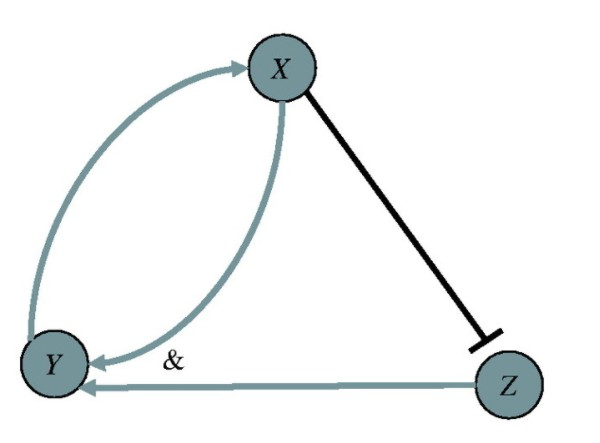
\includegraphics[height=4cm]{basicbool}
  \caption{A simple 3 node Boolean network with no signal delay}
  \label{fgr:example}
\end{figure}

\begin{table}[h]
\small
  \caption{\ The values of X,Y and Z at t+1 given XYZ(t)}
  \label{tbl:example}
  \begin{tabular*}{0.5\textwidth}{@{\extracolsep{\fill}}lll}
    \hline
    XYZ(t) & XYZ(t+1) \\
    \hline
    000 & 001 \\
    001 & 001 \\
    010 & 101 \\
    011 & 101 \\
    100 & 000 \\
    101 & 010 \\
    110 & 100 \\
    111 & 110 \\
    \hline
  \end{tabular*}
\end{table}

The paper put forward by Akman et al. compares the Boolean model to data under rather ideal conditions (synchronous, physically relevant photoperiods),  where it performs rather well. This purpose of this paper is to stress test one of these Boolean models put forth under more extreme conditions and parameterizations to determine the model's limitations to further understand the Boolean model's place in GRN modeling.


\section{Methods}

We built a codebase in Matlab to represent and evaluate boolean networks, utilizing a recursive class and evaluation function to represent complex Boolean gates. A matrix was used to represent and store the states of the nodes for each time point, which allowed data from different time points to be accessed during simulation - a necessary piece for signalling delays. Light nodes were implemented to update based on their absolute time step, rather than basing their outputs on stimulus. At the start of any simulation, all states were assumed to be off, and states prior to the start of the simulation (accessed via signalling delays), were assumed to be off. \\
Once this system had been built, it was fairly trivial to implement and simulate a variety of boolean networks. The network we settled on was the 2-loop \textit{Arabidopsis} model (Figure \ref{fgr:network}) given by Akman et al\cite{digiclocks}. We utilized the logic configuration and signaling delays presented, with a little bit of fiddling to ensure that the model produced the results expected by the paper. Once this model was established it was fairly easy to make changes to the parameters in order to experiment with the model's response to change. \\

\begin{figure}[h]
\centering
  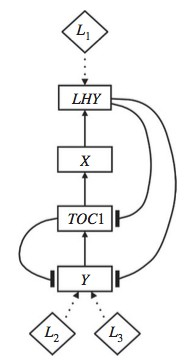
\includegraphics[height=8cm]{network}
  \caption{A simple 3 node Boolean network with no signal delay}
  \label{fgr:network}
\end{figure}

In order to stress the model, we tested all the possible photoperiods that totalled to 24 hours (24hr day, 0 hr night; 23hr day, 1 hr night; etc.) and all the possible photoperiods that totalled to 48 hours. Additionally we ran the model with subsets of lights entirely off (either $L_1$, or $L_2$ \& $L_3$), and tried turning off those subsets of lights in the middle of a simulation. We also tried running the subsets of lights with different periods to examine how the model responded.

\section{Results}

\subsection{Photoperiods}
One of the things we checked was how the model performed when the lights were entirely on or entirely off. When the lights were entirely off, the entire system remained off. When the lights were entirely off, the system produced a fairly simple, biologically plausible cycle, with a period of 28 hours (Figure \ref{fgr:24hr}). \\
For photoperiods totalling to 24 hours within a reasonable window of twelve hours dark, twelve hours light, the model performed about as we expected. The behavior was pretty similar to the general behavior of the model under 12-12(Figure \ref{fgr:12hr}), and we were able to fairly easily understand the causes of any peculiarities. However, for any 24hr period with 18 or more hours of light, the model performed in ways that were clearly not biologically sound (Figure \ref{fgr:18hr}). At all times the nodes were constantly switching back and forth between on and off.\\

\begin{figure}[H]
\centering
  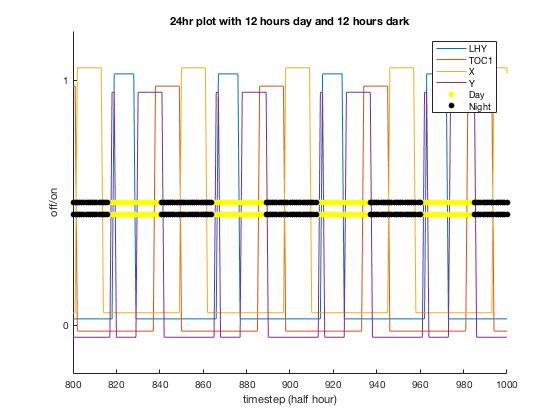
\includegraphics[width=0.50\textwidth,height=3cm]{12hrday}
  \caption{12 hour day}
  \label{fgr:12hr}
\end{figure}
\begin{figure}[H]
\centering
  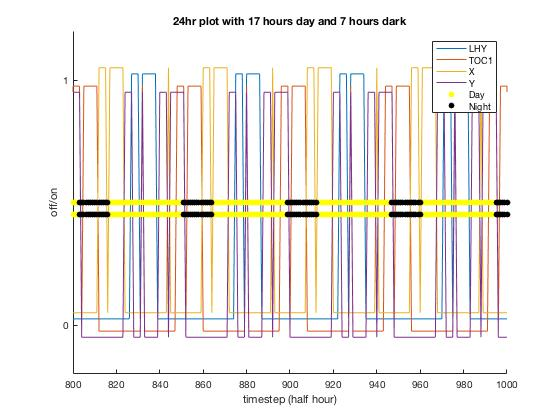
\includegraphics[width=0.5\textwidth,height=3cm]{17hrday}
  \caption{17 hour day}
  \label{fgr:17hr}
\end{figure}
\begin{figure}[H]
\centering
  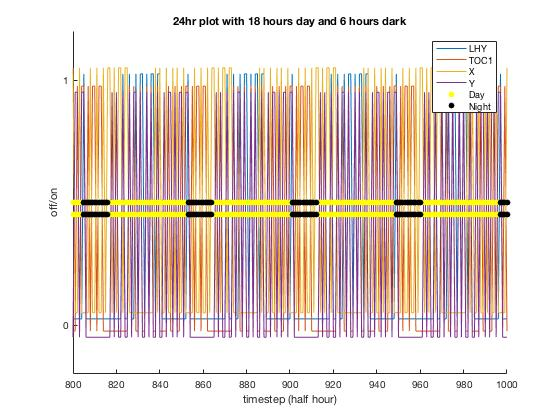
\includegraphics[width=0.5\textwidth,height=3cm]{18hrday}
  \caption{18 hour day}
  \label{fgr:18hr}
\end{figure}
\begin{figure}[H]
\centering
  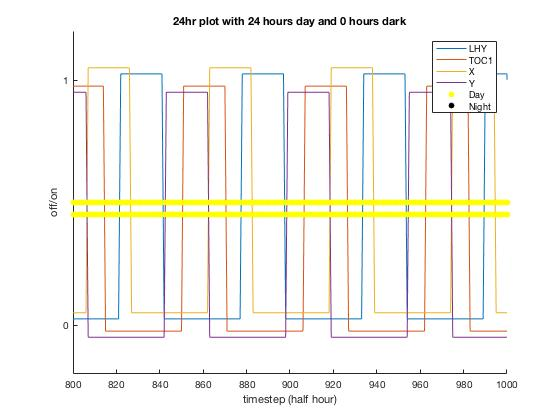
\includegraphics[width=0.5\textwidth,height=3cm]{24hrdayJPG}
  \caption{24 hour day}
  \label{fgr:24hr}
\end{figure}


For photoperiods totalling to 48 hours, we saw some similar behaviors to that of 24hr periods as well as some more unusual things. We noticed that 20 hours was the maximum amount of dark that could occur where genes would be active during the night (Figure \ref{fgr:28hr}). Additionally, with a photoperiod of 42 hours light and 6 hours dark, we discovered a situation where the model acted non-periodically, and noticed a peculiar rapid change in behavior around 430 hours (Figure \ref{fgr:42hr}). 

\newpage


\begin{figure}[H]
\centering
  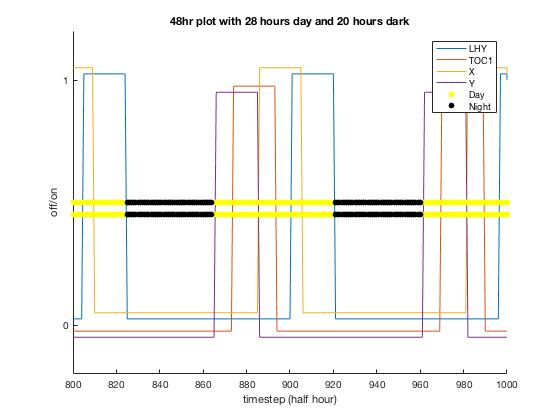
\includegraphics[width=0.5\textwidth,height=3cm]{28d-20n}
  \caption{28hr day, 20 hr night}
  \label{fgr:28hr}
\end{figure}
\begin{figure}[H]
\centering
  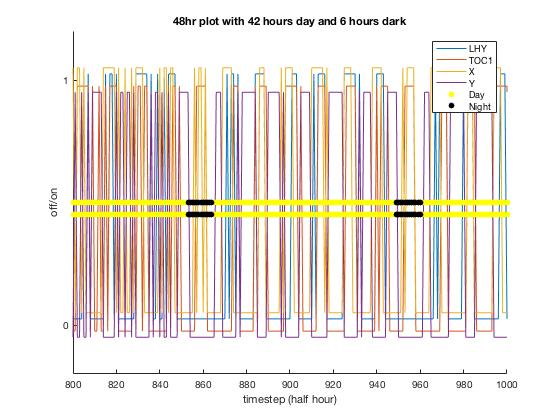
\includegraphics[width=0.5\textwidth,height=3cm]{42d-6n}
  \caption{42hr day, 6 hr night}
  \label{fgr:42hr}
\end{figure}

\subsection{Asynchronous Lights}
For the purposes of this section we grouped $L_1$ as a group of lights and $L_2$ with $L_3$ as a second group of lights. This is because the second group act on the same gene with roughly the same signal delay. We saw in both cases turning off $L_1$ resulted in a new periodic behavior (still 24 hr periodic), one without LHY (Figure \ref{fgr:noL1}). When we turned off the other group of lights ($L_2$ and $L_3$), this resulted in a completely inactive model(Figure \ref{fgr:noL2L3}). \\
\begin{figure}[H]
\centering
  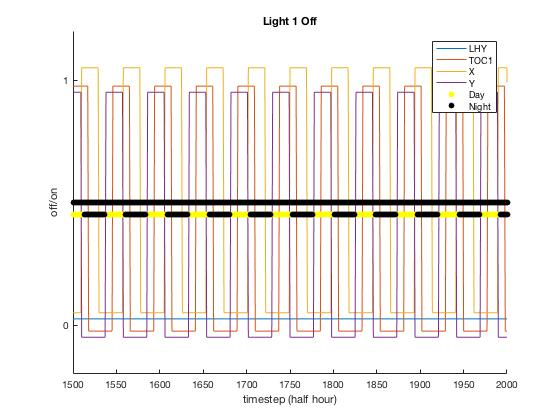
\includegraphics[width=0.5\textwidth,height=3cm]{NoL1}
  \caption{Never turning on L1}
  \label{fgr:noL1}
\end{figure}
\begin{figure}[H]
\centering
  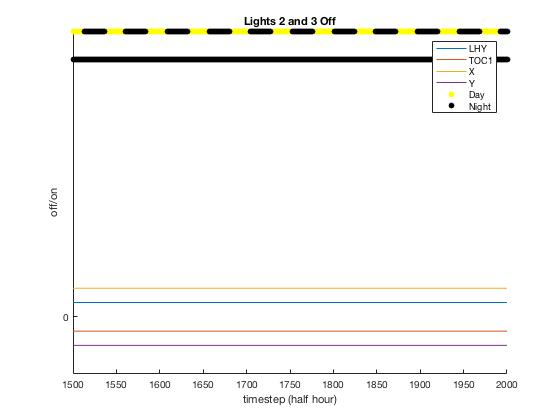
\includegraphics[width=0.5\textwidth,height=3cm]{NoL2L3}
  \caption{Never turning on L2 or L3}
  \label{fgr:noL2L3}
\end{figure}

We then ran these groups of lights concurrently, but with different photo periods. In this case we saw the model still produced periodic behavior, where the period is exactly the least common multiple of the two photoperiods used by the light groups. This claim comes without proper mathematical derivation to show this is always true; however we experimented with many varied photoperiods and each time the resulting period was the LCM of the light photoperiods.

\begin{figure}[H]
\centering
  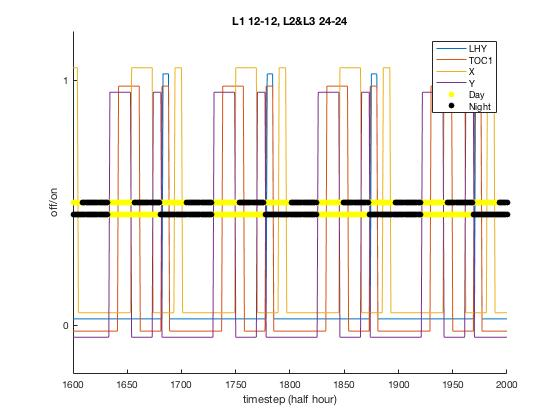
\includegraphics[width=0.5\textwidth,height=3cm]{async1}
  \caption{24hr period + 48hr period = 48hr period}
  \label{fgr:async1}
\end{figure}
\begin{figure}[H]
\centering
  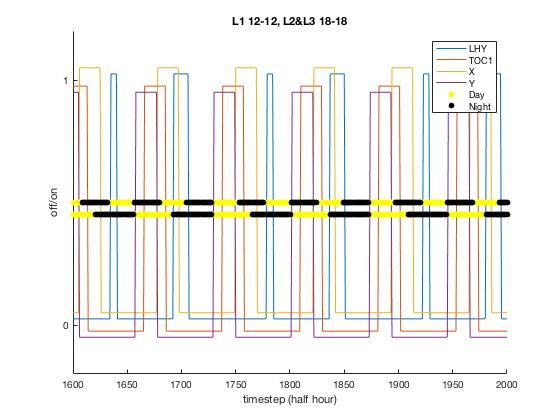
\includegraphics[width=0.5\textwidth,height=3cm]{async2}
  \caption{24hr period + 36hr period = 72hr period}
  \label{fgr:async2}
\end{figure}

\begin{figure}[H]
\centering
  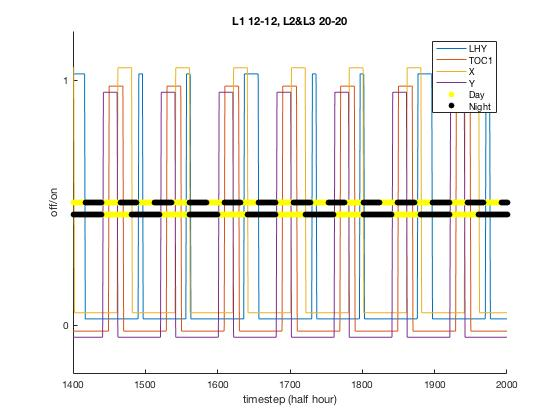
\includegraphics[width=0.5\textwidth,height=3cm]{async3}
  \caption{24hr period + 40hr period = 120hr period}
  \label{fgr:async3}
\end{figure}


\section{Discussion}

When thinking about the photoperiod, some of the results were expected, and some of them were not. It is easy to extrapolate that without light, none of the genes would turn on. Additionally, the constant light produced a fairly reasonable solution that matched what could be expected by a biological equivalent. This isn?t particularly surprising given the model was generated using data produced with lights entirely on. However, the results from 24hr photoperiods with more than 18 hours of light were unexpected. It is difficult to trace why they might be occurring, and as such it is difficult to understand why the change happens so starkly at 18 hours, when at 17 hours the response is fairly normal. \\
We noticed that the 28 hours of day which paired with 20 hours of night at which no genes turn on during the night coincided with the ?natural? period of the system when the lights were just left on. It is unclear at this time whether the 28 hours is more significant than the 20 for dictating if genes remain off during the night. The unusual results produced by 42 hours of light and 6 hours of light are as yet not understood. We were unable to discern why this particular combination might result in chaos, while many similar photoperiods remained periodic.\\
While the model appeared to have trouble working with non-biological photoperiods, the model held up well in the face of asynchronous light behaviors. In the case of turning off $L_1$, we see there still is periodic behavior. This can be expected after seeing that $L_1$ only excites LHY, an inhibitory gene, while gene Y (the main excitatory gene) still activates. Similarly when we turn off the other light group the model produces no behavior because LHY is only inhibitory. This may suggest that not every light node is necessary to construct a control kernel\cite{control} for this model.\\
The model also showed a good ability to regulate sporadic and uneven light inputs into a regulated output. This is behavior we would expect from a circadian system, designed to produce regulated output. The fact that the model produces long period behavior isn't even particularly concerning because it still is pseudo-periodic on a shorter 24hr period. \\
These results went against our initial expectations for this project. We had assumed the model would've taken varied, synchronous photoperiods better than the asynchronous options (including varied, asynchronous photoperiods), but this turned out to be not the case. The underlying reason for this is still unknown and would require a deeper understanding of Boolean network theory than we currently possess.


\section{Conclusions}
Ultimately this paper leaves a lot of room for further exploration of circadian Boolean network models. Because the size of the model made fixing any of the shortcomings we identified unrealistic, the construction of a new more robust model may be in order. Akman also works briefly with a 3-loop \textit{Arabidopsis} model, which may give the model better behavior near the edges of the parameter space. Also, understanding Boolean chaos could help illuminate if the potential chaotic nature of the model means anything for our biological understanding or is simply an artifact of a new modeling method. The success of the model in asynchronous light situations may at first appear simply to be an interesting mathematical exercise; however, there is research to suggest that the light nodes modeled here don?t reflect a full spectrum of light and instead reflect certain wavelengths of light\cite{colors}. If this were the case, this model could prove useful in understanding the operation of circadian systems in environments with light conditions different than a full spectrum (sunrise, deep ocean, etc.)


\section{Acknowledgements}

The authors thank Dmitry Kondrashov for his guidance and advice throughout this project.

%%%END OF MAIN TEXT%%%


%The \balance command can be used to balance the columns on the final page if desired. It should be placed anywhere within the first column of the last page.

%\balance

%If notes are included in your references you can change the title from 'References' to 'Notes and references' using the following command:
%\renewcommand\refname{Notes and references}

%%%REFERENCES%%%
\bibliographystyle{rsc} %the RSC's .bst file
\bibliography{BiologyBib} %You need to replace "rsc" on this line with the name of your .bib file


\end{document}
